Let the rational  numbers $\mathbb{Q}$ be constructed as follows where the rationals are simply all numbers that can be formed as fractions of integers (plus $0$), e.g. $\frac{1}{2}, \frac{3142}{1000}$:

\begin{figure}[H]
    \centering
    \begin{minipage}{0.45\textwidth}
        \centering
        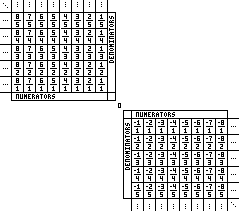
\includegraphics[width=\textwidth]{Illustrations/Rationals_table_no_path.png}
        \caption{The Rationals}
        \label{fig:rationals_indicies_1}
    \end{minipage}
    \hfill
    \begin{minipage}{0.45\textwidth}
        \centering
        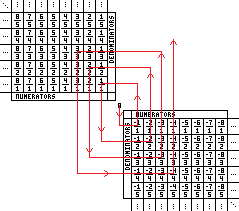
\includegraphics[width=\textwidth]{Illustrations/Rationals_table_with_path.png}
        \caption{Traversable path of The Rationals}
        \label{fig:rationals_indicies_2}
    \end{minipage}
    \caption{The Rationals and how to count them}
\end{figure}

It follows then that by using the path indicated above, you could construct a set $\mathbb{Q} = \{ 0, \frac{1}{1}, \frac{2}{1}, \frac{1}{2}, \frac{3}{1}, \frac{2}{2}, \frac{1}{3}, ...\}$, in this way you can align each member to a corresponding member of $\mathbb{N}$, just as you could with the integers. 
\bigskip

Similarly, for multiplication of $\mathbb{N} \times \mathbb{N}$ giving a cardinality of $\lvert{\mathbb{N}}\rvert \cdot \lvert{\mathbb{N}}\rvert$ you can construct a countable set in the same way, replacing numerators and denominators with the first and second factor of each number.

